% Telos shared preamble.
%
% Every Telos publication is designed to be printed on a home laser printer,
% one sheet at a time, and carried into a boat or a garage. Two constraints
% follow from that and govern everything below:
%
%   1. Pure monochrome. No value is ever a hue. Emphasis is carried by rule
%      weight, fill, and type, never by color, so a grayscale or black-only
%      printer loses nothing.
%   2. Card density. A "one-pager" is a hard contract: the leaf must fit on a
%      single side of US Letter. The layout is therefore tight by default and
%      the environments below are sized to leave room for a plate.

\documentclass[10pt,letterpaper]{article}

\usepackage[margin=0.55in,includefoot,footskip=0.24in]{geometry}
\usepackage[T1]{fontenc}
\usepackage[utf8]{inputenc}
\usepackage{lmodern}
\usepackage{microtype}
\usepackage{array}
\usepackage{booktabs}
\usepackage{longtable}
\usepackage{tabularx}
\usepackage{enumitem}
\usepackage{needspace}
\usepackage{multicol}
\usepackage{ragged2e}
\usepackage{graphicx}
\usepackage{wrapfig}
\usepackage{xcolor}
\usepackage{fancyhdr}
\usepackage{titlesec}
\usepackage{hyperref}
\usepackage[most]{tcolorbox}
\usepackage{tikz}
\usetikzlibrary{arrows.meta,calc,positioning,shapes.geometric,decorations.pathmorphing,patterns,fadings}

% Semantic names are kept so a document reads intelligibly, but every value is
% black, white, or a neutral gray that survives a black-only print driver.
\definecolor{telosink}{gray}{0}
\definecolor{telospaper}{gray}{1}
\definecolor{telosrule}{gray}{0.35}
\definecolor{telosfill}{gray}{0.90}
\definecolor{telosdeep}{gray}{0.72}
\definecolor{telosmute}{gray}{0.45}

\hypersetup{hidelinks,pdfborder={0 0 0}}

% Keep an unchanged source byte-reproducible across rebuilds: no build-clock
% creation date and no random trailer ID.
\pdfinfoomitdate=1
\pdftrailerid{}

\setlength{\parindent}{0pt}
\setlength{\parskip}{0.42em}
\setlength{\tabcolsep}{4pt}
\setlength{\columnsep}{1.1em}
\renewcommand{\arraystretch}{1.18}
\setlist[itemize]{leftmargin=1.15em,itemsep=0.12em,topsep=0.2em,parsep=0pt}
\setlist[enumerate]{leftmargin=1.5em,itemsep=0.18em,topsep=0.2em,parsep=0pt}
\setlist[description]{leftmargin=0pt,itemsep=0.16em,topsep=0.2em,parsep=0pt,
  font=\normalfont\bfseries}

% ---------------------------------------------------------------------------
% Document identity. Each leaf declares these before \begin{document} so the
% running head, the colophon, and the PDF metadata all agree.
% ---------------------------------------------------------------------------
\newcommand{\TelosProject}{Telos}
\newcommand{\TelosDocTitle}{}
\newcommand{\TelosDocSubtitle}{}
\newcommand{\TelosRevision}{}

\newcommand{\telosmeta}[4]{%
  \renewcommand{\TelosProject}{#1}%
  \renewcommand{\TelosDocTitle}{#2}%
  \renewcommand{\TelosDocSubtitle}{#3}%
  \renewcommand{\TelosRevision}{#4}%
  \hypersetup{pdftitle={#2},pdfsubject={#3; version #4},
    pdfkeywords={Telos, version #4},pdfauthor={Telos}}%
}

\pagestyle{fancy}
\fancyhf{}
\renewcommand{\headrulewidth}{0pt}
\renewcommand{\footrulewidth}{0.4pt}
\fancyfoot[L]{\footnotesize\textsc{\TelosProject}}
\fancyfoot[C]{\footnotesize\TelosDocTitle}
\fancyfoot[R]{\footnotesize\thepage}

% The first page of a one-pager carries the masthead instead of a running foot,
% so its footer is the compact provenance line.
\fancypagestyle{telosfirst}{%
  \fancyhf{}%
  \renewcommand{\headrulewidth}{0pt}%
  \renewcommand{\footrulewidth}{0.4pt}%
  \fancyfoot[L]{\footnotesize\textsc{\TelosProject}}%
  \fancyfoot[C]{\footnotesize\TelosRevision}%
  \fancyfoot[R]{\footnotesize\thepage}%
}

% ---------------------------------------------------------------------------
% Masthead. A heavy rule, the title, a light subtitle, a thin rule. The
% optional argument is a right-aligned tag (a species' scientific name, a
% lesson number) that sits on the title's baseline.
% ---------------------------------------------------------------------------
\newcommand{\telosmasthead}[1][]{%
  \thispagestyle{telosfirst}%
  \begingroup
  \setlength{\parskip}{0pt}%
  \noindent\rule{\linewidth}{1.6pt}\par
  \vspace{0.30em}
  \noindent
  \begin{minipage}[b]{0.66\linewidth}
    \raggedright{\LARGE\bfseries\TelosDocTitle}
  \end{minipage}%
  \hfill
  \begin{minipage}[b]{0.32\linewidth}
    \raggedleft{\small\itshape #1}
  \end{minipage}\par
  \vspace{0.18em}
  \noindent{\small\TelosDocSubtitle}\par
  \vspace{0.28em}
  \noindent\rule{\linewidth}{0.4pt}\par
  \endgroup
  \vspace{0.35em}
}

% ---------------------------------------------------------------------------
% Headings. Compact, small-caps, rule-anchored — a card has no room for the
% article class's default vertical air.
% ---------------------------------------------------------------------------
\titleformat{\section}{\normalfont\large\bfseries}{}{0pt}{}[\vspace{-0.55em}\rule{\linewidth}{0.4pt}]
\titlespacing*{\section}{0pt}{0.85em}{0.35em}
\titleformat{\subsection}{\normalfont\normalsize\bfseries}{}{0pt}{}
\titlespacing*{\subsection}{0pt}{0.6em}{0.2em}
\titleformat{\subsubsection}{\normalfont\small\bfseries\scshape}{}{0pt}{}
\titlespacing*{\subsubsection}{0pt}{0.45em}{0.12em}

% A short run-in heading for card interiors that must not consume a full line.
\newcommand{\telosrubric}[1]{\textbf{#1}\enspace}

% Cross-reference helper. Every Telos project is a set of loose printed sheets,
% so a reference names the sheet rather than a page number.
\newcommand{\sheetref}[1]{\textit{see the \textbf{#1} sheet}}

% Which decision, ADR or sheet governs the paragraph you are reading. A reader
% who disagrees with an instruction should be able to find the reasoning behind
% it rather than having to take it on trust.
\newcommand{\governedby}[1]{{\footnotesize\textsc{governed by #1}}}

% ---------------------------------------------------------------------------
% Quantities. siunitx is not in this TeX Live split, and the guides need only a
% fixed thin space and upright units, so define that directly rather than take
% a package dependency the documented install would not satisfy.
%   \qty{9}{kV}  ->  9 kV        \unitof{kV}  ->  kV
% ---------------------------------------------------------------------------
\newcommand{\unitof}[1]{\ensuremath{\mathrm{#1}}}
\newcommand{\qty}[2]{#1\,\unitof{#2}}
\newcommand{\numrange}[2]{#1\,--\,#2}
\newcommand{\qtyrange}[3]{#1\,--\,#2\,\unitof{#3}}
% Inches and feet appear constantly in the fishing guide; keep one spelling.
\newcommand{\inch}[1]{#1\,in}
\newcommand{\feet}[1]{#1\,ft}

% ---------------------------------------------------------------------------
% Cards and boxes.
% ---------------------------------------------------------------------------

% Titled card with a hairline frame. The default card for facts a reader looks
% up rather than reads through.
\newtcolorbox{teloscard}[1]{
  enhanced, breakable,
  colback=telospaper, colframe=telosink, colbacktitle=telospaper,
  coltitle=telosink,
  boxrule=0.5pt, sharp corners,
  left=6pt, right=6pt, top=4pt, bottom=4pt,
  toptitle=3pt, bottomtitle=3pt, titlerule=0.4pt,
  before skip=6pt, after skip=6pt,
  title={#1}, fonttitle=\small\bfseries
}

% Untitled left-ruled block: hierarchy without a redundant label.
\newtcolorbox{telosframe}{
  enhanced, breakable,
  colback=telospaper, frame hidden, boxrule=0pt, sharp corners,
  borderline west={1.3pt}{0pt}{telosink},
  left=8pt, right=2pt, top=3pt, bottom=3pt,
  before skip=6pt, after skip=6pt
}

% Filled emphasis panel — the "read this first" block. The 10% fill stays
% legible under a cheap laser toner curve and still reads as distinct.
\newtcolorbox{telospanel}[1]{
  enhanced, breakable,
  colback=telosfill, colframe=telosink, colbacktitle=telosfill,
  coltitle=telosink,
  boxrule=0.5pt, sharp corners,
  left=6pt, right=6pt, top=4pt, bottom=4pt,
  toptitle=3pt, bottomtitle=3pt, titlerule=0.4pt,
  before skip=6pt, after skip=6pt,
  title={#1}, fonttitle=\small\bfseries
}

% Hazard block. Deliberately the heaviest object on any page: a 1.4pt frame
% plus a solid title bar. Nothing else in Telos is allowed to look like this,
% so a reader skimming a lesson cannot mistake it for ordinary emphasis.
\newtcolorbox{teloshazard}[1]{
  enhanced, breakable,
  colback=telospaper, colframe=telosink,
  colbacktitle=telosink, coltitle=telospaper,
  boxrule=1.4pt, sharp corners,
  left=6pt, right=6pt, top=5pt, bottom=5pt,
  toptitle=3pt, bottomtitle=3pt,
  before skip=8pt, after skip=8pt,
  title={\MakeUppercase{#1}}, fonttitle=\small\bfseries
}

% A stop-and-check gate. Used before anything destructive, and before anything
% that would be expensive to discover later. Shared by every project that has
% a procedure someone could get hurt following carelessly.
\newtcolorbox{gate}[1]{
  enhanced, breakable,
  colback=telospaper, colframe=telosink,
  boxrule=1.0pt, sharp corners,
  left=6pt, right=6pt, top=4pt, bottom=4pt,
  toptitle=3pt, bottomtitle=3pt, titlerule=0.4pt,
  before skip=7pt, after skip=7pt,
  colbacktitle=telospaper, coltitle=telosink,
  title={\MakeUppercase{#1}}, fonttitle=\small\bfseries
}

% ---------------------------------------------------------------------------
% Rating dots. A five-step scale that prints identically in black-only: filled
% versus open circles, never a shaded bar.
% ---------------------------------------------------------------------------
\newcommand{\telosdot}{\tikz[baseline=-0.42ex]\fill[telosink] (0,0) circle (0.28ex);}
\newcommand{\telosopendot}{\tikz[baseline=-0.42ex]\draw[telosink,line width=0.28pt] (0,0) circle (0.28ex);}
\makeatletter
\newcounter{telos@rate}
\newcommand{\telosrating}[1]{%
  \begingroup
  \setcounter{telos@rate}{0}%
  \@whilenum\value{telos@rate}<#1\do{\telosdot\kern0.22em\stepcounter{telos@rate}}%
  \@whilenum\value{telos@rate}<5\do{\telosopendot\kern0.22em\stepcounter{telos@rate}}%
  \endgroup
}
\makeatother

% ---------------------------------------------------------------------------
% Tables.
%
% tabularx reads its body by scanning for a literal \end{tabularx}, so it can
% never be wrapped in a \newenvironment. Documents therefore open tabularx and
% longtable directly and take their house style from these column types and the
% booktabs rules. The one exception is the fact strip below, which is built on
% plain tabular precisely so it *can* be an environment.
% ---------------------------------------------------------------------------
\newcolumntype{L}{>{\raggedright\arraybackslash}X}
\newcolumntype{R}{>{\raggedleft\arraybackslash}X}
\newcolumntype{C}{>{\centering\arraybackslash}X}
\newcolumntype{B}{>{\bfseries\raggedright\arraybackslash}X}
\newcolumntype{N}{>{\raggedright\arraybackslash}p{0.16\linewidth}}

% Key/value fact strip. Two flush columns of short lookups; the label column is
% a fixed fraction so a stack of cards aligns across the whole guide.
\newenvironment{telosfacts}[1][0.24]
  {\begingroup\small
   \setlength{\parskip}{0pt}%
   \renewcommand{\arraystretch}{1.25}%
   \begin{tabular}{@{}>{\bfseries\raggedright\arraybackslash}p{\dimexpr#1\linewidth\relax}@{\hspace{0.7em}}>{\raggedright\arraybackslash}p{\dimexpr\linewidth-#1\linewidth-0.7em\relax}@{}}}
  {\end{tabular}\par\endgroup}
\newcommand{\telosfact}[2]{#1 & #2\\}

% ---------------------------------------------------------------------------
% Seasonal / diurnal activity bar.
%
% \telosseasonbar{4,3,2,1,1,2,3,3,4,5,4,3} draws a twelve-cell month strip
% where each value 0-5 is a fill height. Height, not gray value, carries the
% signal, so it is exact under any toner curve; the cell is outlined either way
% so an empty month is still visibly a month.
% ---------------------------------------------------------------------------
\newcommand{\telosseasonlabels}{J,F,M,A,M,J,J,A,S,O,N,D}
\newcommand{\telosseasonbar}[1]{%
  \begingroup
  \begin{tikzpicture}[x=1.25em,y=2.1ex,baseline=0pt]
    \foreach \v [count=\i from 0] in {#1} {
      \draw[telosrule,line width=0.3pt] (\i,0) rectangle (\i+0.86,5);
      \ifnum\v>0
        \fill[telosink] (\i,0) rectangle (\i+0.86,\v);
      \fi
    }
    \foreach \m [count=\i from 0] in \telosseasonlabels {
      \node[font=\tiny,anchor=north,inner sep=1.2pt] at (\i+0.43,-0.1) {\m};
    }
  \end{tikzpicture}%
  \endgroup
}

% Four-cell day-part strip: dawn, midday, dusk, night.
\newcommand{\telosdaylabels}{Dawn,Mid,Dusk,Night}
\newcommand{\telosdaybar}[1]{%
  \begingroup
  \begin{tikzpicture}[x=2.9em,y=2.1ex,baseline=0pt]
    \foreach \v [count=\i from 0] in {#1} {
      \draw[telosrule,line width=0.3pt] (\i,0) rectangle (\i+0.92,5);
      \ifnum\v>0
        \fill[telosink] (\i,0) rectangle (\i+0.92,\v);
      \fi
    }
    \foreach \m [count=\i from 0] in \telosdaylabels {
      \node[font=\tiny,anchor=north,inner sep=1.2pt] at (\i+0.46,-0.1) {\m};
    }
  \end{tikzpicture}%
  \endgroup
}

% A bar needs vertical room for its labels when it sits in a fact strip.
\newcommand{\telosbarrow}[1]{\rule{0pt}{4.2ex}#1\rule[-1.6ex]{0pt}{1.6ex}}

% ---------------------------------------------------------------------------
% Plates. A species or apparatus illustration with a caption rule beneath it.
% \telosplate{width fraction}{file}{caption}
% ---------------------------------------------------------------------------
\newcommand{\telosplate}[3]{%
  \begingroup
  \centering
  \includegraphics[width=#1\linewidth]{#2}\par
  \vspace{0.15em}
  \begin{minipage}{#1\linewidth}
    \rule{\linewidth}{0.4pt}\par
    \vspace{0.1em}
    {\footnotesize #3\par}
  \end{minipage}\par
  \endgroup
  \vspace{0.3em}
}

% TikZ drawing conventions shared by every rig, knot, and circuit diagram.
\tikzset{
  telos line/.style={draw=telosink,line width=0.7pt},
  telos hair/.style={draw=telosink,line width=0.35pt},
  telos heavy/.style={draw=telosink,line width=1.2pt},
  telos node/.style={draw=telosink,fill=telospaper,align=center,inner sep=4pt,font=\small},
  telos emphasis/.style={draw=telosink,line width=1.2pt,fill=telospaper,align=center,
    inner sep=4pt,font=\small\bfseries},
  telos label/.style={font=\scriptsize,inner sep=1.5pt},
  telos arrow/.style={-{Stealth[length=1.8mm]},draw=telosink,line width=0.6pt},
  telos dim/.style={|<->|,draw=telosink,line width=0.35pt},
  telos water/.style={draw=telosrule,line width=0.4pt,decorate,
    decoration={snake,amplitude=0.4mm,segment length=3mm}},
}

% ---------------------------------------------------------------------------
% Lesson furniture
% ---------------------------------------------------------------------------

% \lessonhead{number}{time}{who does what}
\newcommand{\lessonhead}[3]{%
  \par\noindent
  \begin{minipage}{\linewidth}
    \rule{\linewidth}{0.4pt}\par
    \vspace{0.3em}
    {\small\textbf{Lesson #1}\quad$\cdot$\quad #2\quad$\cdot$\quad #3\par}
    \vspace{0.25em}
    \rule{\linewidth}{0.4pt}
  \end{minipage}\par
  \vspace{0.5em}}

% The materials list. Two columns of short lines; a lesson that needs a long
% shopping list is a lesson that has not been thought through.
\newenvironment{materials}
  {\begin{telospanel}{What you need}\begin{multicols}{2}
   \begin{itemize}[leftmargin=1em,itemsep=0.05em,topsep=0pt]}
  {\end{itemize}\end{multicols}\end{telospanel}}

% The four rubrics every lesson carries, in the same order every time:
% what you are about to see, what to do, what it means, and what to ask.
\newcommand{\lessonsection}[1]{\section*{#1}\vspace{-0.35em}\rule{\linewidth}{0.4pt}\vspace{0.2em}}

% A prediction box. The point of the curriculum is that they commit to an
% answer before the demonstration, not after.
\newtcolorbox{predict}{
  enhanced, breakable,
  colback=telospaper, colframe=telosink,
  boxrule=0.5pt, sharp corners,
  left=6pt, right=6pt, top=4pt, bottom=4pt,
  before skip=6pt, after skip=6pt,
  borderline west={2.2pt}{0pt}{telosink},
  title={\small\bfseries Predict first}, fonttitle=\small\bfseries,
  colbacktitle=telospaper, coltitle=telosink,
  toptitle=3pt, bottomtitle=3pt, titlerule=0.4pt,
}

% ---------------------------------------------------------------------------
% Colophon. Rendered once, at the end of the last page, in the recovered footer
% area so it never creates a page of its own.
% ---------------------------------------------------------------------------
\newif\ifTelosColophonRendered
\newcommand{\TelosColophonExtra}{}
\newcommand{\TelosColophon}{%
  \ifTelosColophonRendered\else
  \global\TelosColophonRenderedtrue
  \par
  \enlargethispage{0.5in}%
  \vspace{0.3em}%
  \begingroup
  \setlength{\parskip}{0pt}%
  \begin{minipage}{\linewidth}
  \rule{\linewidth}{0.35pt}\par
  \vspace{0.3em}%
  \fontsize{7}{8.2}\selectfont
  \textbf{Telos.} \TelosProject{} — \TelosDocTitle. Revised \TelosRevision.
  \TelosColophonExtra{}
  Project-created text and diagrams are licensed \href{https://creativecommons.org/licenses/by/4.0/}{CC BY 4.0}.
  Incorporated public-domain artwork remains public domain and is credited on
  the plate it appears with. See \texttt{LICENSE} and \texttt{CREDITS.md} in the
  source. Nothing here is professional advice; verify current regulations and
  follow the stated safety procedure.
  \end{minipage}
  \endgroup
  \fi
}
\AtEndDocument{\TelosColophon}

% ChatGPT edition map primitives. Original monochrome drawings; no Claude map
% geometry or generated output is imported.
\tikzset{
  cgshore/.style={draw=black,line width=1pt,fill=white},
  cgten/.style={draw=black,line width=.5pt},
  cgtwenty/.style={draw=black,line width=.42pt},
  cgforty/.style={draw=black,line width=.35pt,dash pattern=on 4pt off 1.5pt},
  cgsixty/.style={draw=black,line width=.32pt,dash pattern=on 2pt off 1.2pt},
  cgspot/.style={circle,fill=black,text=white,minimum size=3.3mm,inner sep=0pt,
    font=\fontsize{6}{6}\selectfont\bfseries},
  cgdepth/.style={fill=white,inner sep=.6pt,font=\fontsize{5.5}{6}\selectfont},
  cgnote/.style={fill=white,inner sep=1pt,font=\fontsize{6}{7}\selectfont}
}
\newcommand{\cgspot}[3]{\node[cgspot] at (#1,#2) {#3};}
\newcommand{\cgnorth}[2]{%
  \draw[-{Stealth[length=1.8mm]},line width=.5pt] (#1,#2) -- ++(0,.65);
  \node[font=\scriptsize\bfseries,anchor=south] at (#1,#2+.65) {N};}
\newcommand{\cgscale}[4]{%
  \draw[line width=.5pt] (#1,#2) -- ++(#3,0);
  \draw[line width=.5pt] (#1,#2-.07) -- ++(0,.14);
  \draw[line width=.5pt] (#1+#3,#2-.07) -- ++(0,.14);
  \node[font=\fontsize{5.5}{6}\selectfont,anchor=north] at (#1+#3/2,#2-.08) {#4};}

\telosmeta{Lake Country Fishing}{North Lake}
  {WBIC 850800 --- independent field sheet}{2026-07-26}

\begin{document}
\telosmasthead[Waukesha County, Wisconsin]

North is a deep drainage lake with two strongly defined basins joined through
a narrow structural corridor. The historical survey shows abrupt edges, small
humps and a south neck toward Mud Lake. Use those shapes as hypotheses; confirm
today's depth, vegetation, access and hazards yourself.

\begin{telosfacts}[0.19]
\telosfact{Identity}{WBIC 850800; 440 acres}
\telosfact{Depth}{78.4 ft maximum}
\telosfact{Bottom}{50\% sand; 30\% gravel; 20\% muck}
\telosfact{Type}{Drainage lake; DNR classifies it eutrophic}
\telosfact{Current DNR fish record}{Panfish, largemouth bass, smallmouth bass,
 northern pike and walleye}
\telosfact{Access}{DNR does not list a numbered landing on the facts page.
 Confirm legal public access before arrival; a historical road is not permission}
\end{telosfacts}

\begin{center}
\begin{tikzpicture}[x=.78cm,y=.78cm]
% Independent generalization of the 1898/1941 DNR sheet, checked against NAIP.
\path[cgshore]
 (4.7,12.5)..controls(3.5,12.7)and(2.9,11.8)..(2.8,10.7)
 ..controls(2.7,9.6)and(3.0,8.8)..(2.5,7.8)
 ..controls(2.1,7.0)and(1.1,7.0)..(.8,6.1)
 ..controls(.4,5.2)and(.6,3.8)..(1.4,3.3)
 ..controls(2.2,2.8)and(3.0,3.4)..(3.4,4.2)
 ..controls(3.7,4.8)and(4.1,4.3)..(4.4,3.7)
 ..controls(4.7,3.0)and(4.2,2.2)..(4.6,1.4)
 ..controls(5.1,.7)and(5.8,1.1)..(6.4,1.2)
 ..controls(7.0,1.4)and(7.2,2.4)..(7.4,3.4)
 ..controls(7.6,4.5)and(7.4,5.7)..(7.5,6.8)
 ..controls(7.7,8.0)and(7.6,9.3)..(7.8,10.5)
 ..controls(8.0,11.5)and(7.3,12.3)..(6.4,12.2)
 ..controls(5.7,12.1)and(5.4,12.7)..(4.7,12.5)--cycle;
\draw[cgten]
 (4.6,12.1)..controls(3.5,12.1)and(3.2,11.1)..(3.2,10.0)
 ..controls(3.1,8.8)and(3.5,7.6)..(3.0,6.7)
 ..controls(2.7,6.2)and(1.6,6.8)..(1.2,5.9)
 ..controls(.8,5.0)and(1.2,3.9)..(2.0,3.7)
 ..controls(2.9,3.5)and(3.4,4.6)..(3.8,5.2)
 ..controls(4.3,5.8)and(4.7,4.6)..(4.9,3.8)
 ..controls(5.1,3.0)and(4.6,2.1)..(5.2,1.7)
 ..controls(6.0,1.4)and(6.8,1.9)..(6.9,3.1)
 ..controls(7.1,4.3)and(6.9,5.6)..(7.1,6.8)
 ..controls(7.2,8.0)and(7.0,9.2)..(7.3,10.4)
 ..controls(7.5,11.3)and(6.8,11.8)..(6.0,11.7)
 ..controls(5.4,11.6)and(5.1,12.1)..(4.6,12.1)--cycle;
\draw[cgtwenty]
 (4.7,11.7)..controls(3.8,11.5)and(3.6,10.4)..(3.7,9.3)
 ..controls(3.8,8.2)and(3.7,7.1)..(3.4,6.4)
 ..controls(3.0,5.8)and(2.7,6.5)..(2.0,6.1)
 ..controls(1.3,5.7)and(1.4,4.4)..(2.1,4.1)
 ..controls(3.0,3.8)and(3.4,5.3)..(4.0,5.7)
 ..controls(4.7,6.2)and(5.1,5.0)..(5.3,4.0)
 ..controls(5.5,3.1)and(5.1,2.4)..(5.7,2.1)
 ..controls(6.5,2.0)and(6.6,3.2)..(6.6,4.2)
 ..controls(6.6,5.5)and(6.5,6.8)..(6.7,8.0)
 ..controls(6.9,9.2)and(6.7,10.6)..(6.2,11.2)
 ..controls(5.8,11.7)and(5.2,11.8)..(4.7,11.7)--cycle;
\draw[cgforty]
 (4.9,10.9)..controls(4.2,10.4)and(4.4,9.1)..(4.2,8.0)
 ..controls(4.0,6.9)and(4.7,6.1)..(5.2,5.3)
 ..controls(5.8,4.4)and(5.4,3.5)..(5.9,2.9)
 ..controls(6.3,3.6)and(6.0,5.1)..(6.2,6.2)
 ..controls(6.5,7.6)and(6.5,9.3)..(6.0,10.4)
 ..controls(5.7,11.1)and(5.3,11.2)..(4.9,10.9)--cycle;
\draw[cgsixty]
 (5.1,10.1)..controls(4.8,9.1)and(5.0,8.0)..(5.0,7.0)
 ..controls(5.0,6.2)and(5.7,5.3)..(5.8,4.5)
 ..controls(6.1,5.7)and(5.9,7.0)..(6.1,8.2)
 ..controls(6.2,9.4)and(5.8,10.2)..(5.1,10.1)--cycle;
\draw[cgforty] (1.9,5.8)..controls(1.4,5.2)and(1.7,4.3)..(2.3,4.2)
 ..controls(2.9,4.3)and(3.1,5.3)..(2.7,5.8)--cycle;
\draw[cgsixty] (2.0,5.3)..controls(1.8,4.8)and(2.1,4.4)..(2.5,4.5)
 ..controls(2.9,4.9)and(2.6,5.4)..(2.0,5.3)--cycle;
\node[cgdepth] at (5.45,8.2) {78.4};
\node[cgdepth] at (2.35,4.85) {77.6};
\node[cgdepth] at (6.05,3.1) {65};
\cgspot{4.05}{11.25}{1}\cgspot{6.8}{10.6}{2}\cgspot{4.25}{7.2}{3}
\cgspot{1.35}{5.7}{4}\cgspot{2.25}{4.8}{5}\cgspot{3.8}{5.5}{6}
\cgspot{5.7}{5.2}{7}\cgspot{6.2}{2.8}{8}\cgspot{4.85}{1.4}{9}
\node[draw=black,fill=white,minimum size=3mm,inner sep=0pt,font=\scriptsize\bfseries]
 at (6.6,12.3) {?};
\node[cgnote,anchor=west] at (6.82,12.3) {verify access};
\cgnorth{8.1}{11.3}\cgscale{.5}{.25}{1.45}{0.25 mile}
\end{tikzpicture}


\begin{minipage}{.93\linewidth}
\fontsize{8}{9.3}\selectfont
\textbf{Generalized depth contours:} solid 10 ft; widely dashed 20 ft; long dash 40 ft;
short dash 60 ft; labeled historical soundings. \textbf{Not for navigation.}
Independently drafted from the Wisconsin Conservation Department sheet compiled
in 1898 and revised in 1941; current shoreline/access context checked against
2024 USDA/FSA NAIP aerial orthophotography. No imagery is reproduced. A question
mark means access must be independently verified.
\end{minipage}
\end{center}

\newpage
\section{Nine places to test, not promises}

\begin{longtable}{@{}p{.04\linewidth}p{.19\linewidth}p{.34\linewidth}p{.37\linewidth}@{}}
\toprule
\# & \textbf{Area} & \textbf{Why test it} & \textbf{First pass}\\
\midrule\endhead
1 & North flat & Broad shallow water meets the main basin. &
 Search for the current weed edge and bait; cover it without crossing beds.\\
2 & Northeast break & Contours crowd the eastern shore. &
 Keep the boat outside, cast uphill, and identify contact depth.\\
3 & Central channel edge & A structural corridor joins north and south water. &
 Scan both lips for bait or fish before committing.\\
4 & West-lobe rim & A sharp outside curve enters the western basin. &
 Work from the shallow crown down through 20--40 ft.\\
5 & West-lobe basin & A compact 77.6-ft bowl offers nearby deep water. &
 Scan for suspended life; do not fish empty depth.\\
6 & Central saddle & The pinch between lobes concentrates routes, not
 necessarily fish. & Make controlled passes on each side and compare.\\
7 & Southeast hump & Small isolated structure breaks the main basin wall. &
 Circle it to find the steep and windward faces.\\
8 & South basin edge & A 65-ft pocket meets the lower taper. &
 Check low light and seasonal transitions; follow bait, not the printed number.\\
9 & South neck & Shallow constriction toward Mud Lake. &
 Verify navigation, access and regulations before fishing moving-water edges.\\
\bottomrule
\end{longtable}

\section{North Lake sequence}

\begin{enumerate}
\item Confirm legal public access before towing or carrying a craft to the
water. Read every posted ordinance and high-water notice.
\item Sample one lobe, the saddle and one eastern break. A lake-wide pattern
needs repeated depth/bottom evidence, not one bite.
\item Because DNR classifies North as eutrophic, let current vegetation,
oxygen, clarity and bait observations override the antique contour sheet.
\item DNR records Eurasian water-milfoil and zebra mussel. Inspect, remove and
drain before transport; never move live fish away from the water.
\end{enumerate}

\begin{teloshazard}{Access and contours require verification}
The source map began in 1898 and was revised in 1941. Its north road label does
not establish a present public landing. Neither this redrawing nor an aerial
image grants access. Confirm ownership, legal access, depth and hazards through
current official information and direct observation.
\end{teloshazard}

\newpage
\section{Read two basins as a connected system}

\begin{center}
\begin{tikzpicture}[x=1cm,y=1cm]
\draw[cgten] (0,0) ellipse (1.45 and .9);
\draw[cgtwenty] (0,0) ellipse (1.05 and .6);
\draw[cgforty] (0,0) ellipse (.58 and .3);
\draw[cgten] (5.4,0) ellipse (1.7 and 1.05);
\draw[cgtwenty] (5.4,0) ellipse (1.25 and .7);
\draw[cgforty] (5.4,0) ellipse (.72 and .38);
\draw[cgten] (1.42,.12)..controls(2.4,.38)and(3.1,.38)..(3.72,.12);
\draw[cgtwenty] (1.0,-.18)..controls(2.25,-.45)and(3.3,-.45)..(4.18,-.18);
\node[font=\small] at (0,1.25) {west lobe};
\node[font=\small] at (5.4,1.42) {main basin};
\node[font=\small,align=center] at (2.65,.92) {saddle / corridor};
\draw[-{Latex}] (2.65,.78)--(2.65,.25);
\end{tikzpicture}
\end{center}

\begin{enumerate}
\item On the lake map, draw a route that samples location 5, then 6, then 3
without crossing the same contour more than necessary.
\item At location 6, mark one station on each lip of the saddle. Predict which
lip receives today's wind and which offers the quieter measurement station.
\item Compare locations 2 and 4. Circle the one with tighter contour spacing;
write how much boat-position error you can tolerate before a cast misses the
break.
\item Trace the shallowest apparent route between locations 8 and 9. List two
reasons the historical route may not be safe or navigable now.
\end{enumerate}

\begin{teloscard}{Prediction before launch}
If the two lobes differ, I expect \rule{1.55in}{.4pt} to have clearer /
warmer water because \rule{2.2in}{.4pt}. I will test that claim with
\rule{2in}{.4pt}, not with the first bite alone.
\end{teloscard}

\section{Questions the antique contours cannot settle}
\begin{tabularx}{\linewidth}{@{}X X@{}}
\toprule
\textbf{Question} & \textbf{Direct check}\\
\midrule
Does the central corridor carry bait today? & Scan both lips on reciprocal
headings; require repeatable marks before fishing.\\
Where does living vegetation end? & Measure the outside edge in each lobe;
do not transfer one basin's depth to the other.\\
Is the south neck lawful and passable? & Verify access, signs, depth, current
and obstructions from a safe position; turn back if uncertain.\\
\bottomrule
\end{tabularx}

\newpage
\section{Measure both lobes the same way}

\begin{enumerate}
\item \textbf{Choose four stations.} Use one protected shelf, the west-lobe
rim, one saddle lip and an eastern main-basin break. Identify each by map
number or lawful waypoint.
\item \textbf{Depth.} Stop safely outside traffic. Let sonar stabilize and
repeat the pass on the reciprocal heading. With a marked sounding line, stop
propulsion, wear a PFD and keep line away from hands, feet and propeller.
\item \textbf{Temperature.} Shade the thermometer. Measure surface, 5, 10 and
20 ft where possible, pausing for a stable reading. Use the same depths and
wait time in each lobe; write ``not measured'' instead of estimating.
\item \textbf{Clarity.} From the shaded side, lower a standard black-and-white
Secchi disk to disappearance, then raise it to reappearance. Average the two
depths and repeat. Do not lean overboard in waves.
\item \textbf{Context.} Record wind, sky, recent rain, surface film, vegetation
height, boat traffic and any current through the corridor.
\end{enumerate}

\begin{telospanel}{Compare stations, not impressions}
North's basins may differ on the same day. Use the same tool, units and method
at every station. Temperature and clarity do not by themselves prove adequate
oxygen; measure oxygen with suitable calibrated equipment or leave it unknown.
\end{telospanel}

\subsection{North Lake comparison log}
\renewcommand{\arraystretch}{1.35}
\begin{tabularx}{\linewidth}{@{}p{.11\linewidth}p{.12\linewidth}p{.09\linewidth}
p{.14\linewidth}p{.14\linewidth}X@{}}
\toprule
Date/time & Station/lobe & Depth ft & Temp surface/5/10/20 ft &
Secchi down/up/avg ft & Wind, growth, bait, confidence\\
\midrule
\rule{0pt}{1.05cm}&&&&&\\ \midrule
\rule{0pt}{1.05cm}&&&&&\\ \midrule
\rule{0pt}{1.05cm}&&&&&\\ \midrule
\rule{0pt}{1.05cm}&&&&&\\
\bottomrule
\end{tabularx}
\renewcommand{\arraystretch}{1}

\subsection{Verification questions}
\begin{enumerate}
\item Which measurement differed most between lobes? \rule{1.3in}{.4pt}.
Was the difference larger than repeated-measurement variation?
\item Did reciprocal depth passes agree within \rule{.45in}{.4pt} ft? If not,
name the likely source: slope, weeds, waves, heading or instrument setting.
\item Were repeatable bait marks above, within or below the fastest
temperature change? \rule{1.1in}{.4pt}. What evidence would change that answer?
\end{enumerate}

\newpage
\section{Choose the next test from evidence}

\begin{center}
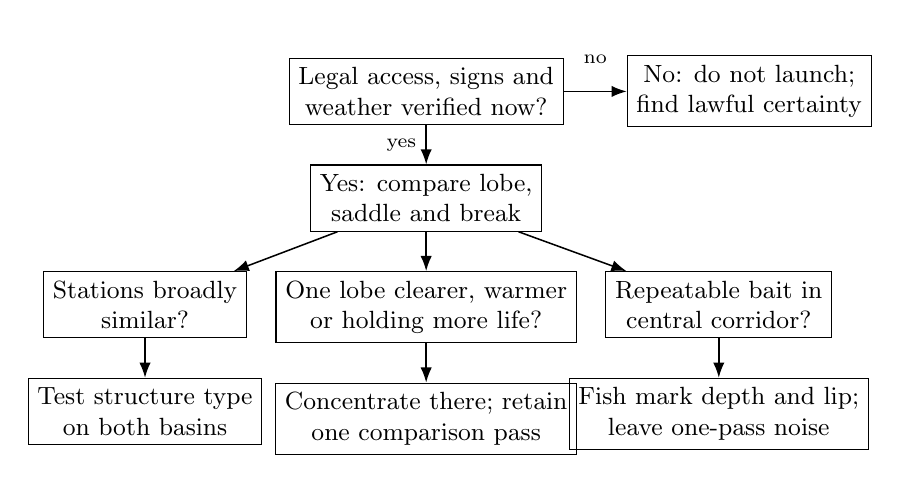
\begin{tikzpicture}[node distance=5mm and 8mm,
every node/.style={draw,align=center,font=\small,minimum height=8mm},
go/.style={-{Latex},line width=.55pt}]
\node (start) {Legal access, signs and\\weather verified now?};
\node[right=of start] (stop) {No: do not launch;\\find lawful certainty};
\node[below=of start] (sample) {Yes: compare lobe,\\saddle and break};
\node[below left=of sample] (same) {Stations broadly\\similar?};
\node[below=of sample] (diff) {One lobe clearer, warmer\\or holding more life?};
\node[below right=of sample] (corr) {Repeatable bait in\\central corridor?};
\node[below=of same] (s1) {Test structure type\\on both basins};
\node[below=of diff] (s2) {Concentrate there; retain\\one comparison pass};
\node[below=of corr] (s3) {Fish mark depth and lip;\\leave one-pass noise};
\draw[go] (start)--node[above,font=\scriptsize,draw=none]{no}(stop);
\draw[go] (start)--node[left,font=\scriptsize,draw=none]{yes}(sample);
\draw[go] (sample)--(same);\draw[go] (sample)--(diff);\draw[go] (sample)--(corr);
\draw[go] (same)--(s1);\draw[go] (diff)--(s2);\draw[go] (corr)--(s3);
\end{tikzpicture}
\end{center}

\subsection{Access and weather gate}
\begin{tabularx}{\linewidth}{@{}p{.31\linewidth}X p{.16\linewidth}@{}}
\toprule
\textbf{Verify on trip day} & \textbf{Evidence seen/heard} & \textbf{Go?}\\
\midrule
Legal public access and permission route && Yes / No\\
Exact-water rules; posted local restrictions && Yes / No\\
Forecast, current radar, wind direction/gusts && Yes / No\\
Lightning, fog, high-water or hazard notice && Yes / No\\
Craft, PFDs, lights, communication and return route && Yes / No\\
\bottomrule
\end{tabularx}

\begin{teloshazard}{Unverified access means no trip}
A road, worn path, map label or online pin is not permission. Confirm the
launch and route through a current authoritative source and the signs on site.
Recheck weather at the water. If access, visibility, waves or restrictions are
uncertain, do not launch or return immediately.
\end{teloshazard}

\subsection{Evidence-to-decision log}
\begin{tabularx}{\linewidth}{@{}p{.13\linewidth}p{.18\linewidth}X X@{}}
\toprule
Time / map \# & Claim tested & Evidence for and against & Next pass and why\\
\midrule
\rule{0pt}{1.2cm}&&&\\ \midrule
\rule{0pt}{1.2cm}&&&\\ \midrule
\rule{0pt}{1.2cm}&&&\\
\bottomrule
\end{tabularx}

\newpage
\section{2026--27 rules printed for departure planning}

\begin{tabularx}{\linewidth}{@{}>{\bfseries}p{.22\linewidth}X@{}}
\toprule
Bass & Harvest May 2, 2026--Mar. 7, 2027; 14 in minimum; 5 daily.
Catch-and-release is open year-round unless otherwise noted.\\
Northern pike & May 2, 2026--Mar. 7, 2027; 26 in minimum; 2 daily.\\
Walleye group & May 2, 2026--Mar. 7, 2027; 18 in minimum; 3 daily.\\
Panfish & Open all year; no minimum; 25 daily.\\
Rock/yellow/white bass & Open all year; no minimum; unlimited.\\
Cisco/whitefish & Open all year; no minimum; 10 daily. Category does not prove presence.\\
Muskellunge & May 2--Dec. 31, 2026, open water only; 40 in minimum; 1 daily.
Category does not prove presence.\\
Motor trolling & Allowed with up to 3 hooks, baits or lures per angler.\\
\bottomrule
\end{tabularx}

\begin{teloshazard}{Recheck before every trip}
These are the Wisconsin DNR lookup results for WBIC 850800 checked 26 July
2026. Verify the exact water, species and date in the live DNR rules. The DNR
says listed regulation categories may not reflect fish actually present.
Posted signs are the definitive practical check for slow-no-wake areas/hours,
high-water restrictions and other local ordinances because the database may lag.
\end{teloshazard}

\section{Evidence boundary}

The current DNR lake record supports panfish, largemouth bass, smallmouth bass,
northern pike and walleye. It does not resolve “panfish” into individual
species. Do not treat regulation-only categories as an inventory. The
provider-neutral evidence record is
\texttt{research/lake-country-fishing/lakes-north.md}.

\section{Primary sources}
\small
Wisconsin DNR Lake Page and historical contour sheet (WBIC 850800); Wisconsin
DNR exact-water fishing-regulation lookup (checked 2026-07-26); Wisconsin DNR
2026--27 regulation changes; USDA/FSA 2024 NAIP via the Wisconsin statewide
imagery service. Full URLs and limitations are in the research file.

\end{document}
